\documentclass[letterpaper,11pt]{article}
\oddsidemargin -1.0cm \textwidth 17.5cm

\usepackage[utf8]{inputenc}
\usepackage[activeacute,spanish]{babel}
\usepackage{amsfonts,setspace}
\usepackage{amsmath}
\usepackage{amssymb, amsmath, amsthm}
\usepackage{comment}
\usepackage{float}
\usepackage{amssymb}
\usepackage{dsfont}
\usepackage{anysize}
\usepackage{multicol}
\usepackage{enumerate}
\usepackage{graphicx}
\usepackage[left=1.5cm,top=1.5cm,right=1.5cm, bottom=1.7cm]{geometry}
\setlength\headheight{1.5em} 
\usepackage{fancyhdr}
\usepackage{multicol}
\usepackage{hyperref}
\usepackage{wrapfig}
\usepackage{subcaption}
\pagestyle{fancy}
\fancyhf{}
\renewcommand{\labelenumi}{\normalsize\bfseries P\arabic{enumi}.}
\renewcommand{\labelenumii}{\normalsize\bfseries (\alph{enumii})}
\renewcommand{\labelenumiii}{\normalsize\bfseries \roman{enumiii})}

\begin{document}

\fancyhead[L]{\itshape{Facultad de Ciencias F\'isicas y Matem\'aticas}}
\fancyhead[R]{\itshape{Universidad de Chile}}

\begin{minipage}{11.5cm}
    \begin{flushleft}
        \hspace*{-0.6cm}\textbf{FI1100-6 Introducción a la Física Moderna}\\
        \hspace*{-0.6cm}\textbf{Profesor:} Diego Mardones\\
        \hspace*{-0.6cm}\textbf{Auxiliares:} Gabriel O\textsc{\char13}Ryan, Camila Sepúlveda, Alejandro Silva\\
        \hspace*{-0.6cm}\textbf{Ayudante:} Sebastián Vargas
    \end{flushleft}
\end{minipage}

\begin{picture}(2,3)
    \put(366, 10){
\includegraphics[scale=0.9]{Imágenes/logo/dfi-fcfm.pdf}}
\end{picture}

\begin{center}
	\LARGE\textbf{Auxiliar \# 5 : Efecto Doppler / Reflexión y refracción de la luz}\\
	\Large{}
\end{center}

\vspace{-1cm}
\begin{enumerate}\setlength{\itemsep}{0.4cm}

\rfoot[]{pág. \thepage}

\item[]

\item Efecto Doppler Doble
La sirena de un patrulla emite una señal de. 300Hz de frecuencia. La patrulla se mueve en dirección hacia una bodega a una velocidad de 30m/s.
\begin{itemize}
    \item ¿Con qué frecuencia escucha la sirena el guardia de la bodega?
    \item ¿Con qué frecuencia escucha el policía dentro de la patrulla la señal que se ha reflejado en la bodega al apagar la sirena?
    \item ¿Como cambian las respuestas anteriores si la patrulla se fuera alejando?
\end{itemize}



\item Leyes de reflexión y refracción desde el principio de Fermat.
Este principio dice que entre todas las trayectorias
posibles entre 2 puntos, la que sigue un rayo de luz es aquélla para el que el tiempo de recorrido es mínimo
Considere los siguientes casos de refracción y reflexión:

\begin{figure}[h]
\centering
\begin{subfigure}{.5\textwidth}
  \centering
  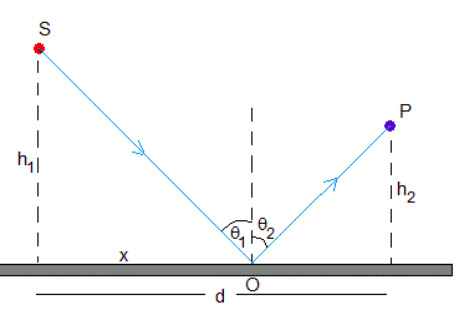
\includegraphics[width=.5\linewidth]{Imágenes/aux5/aux5.png}
  \caption{Reflexión}
  \label{fig:sub1}
\end{subfigure}%
\begin{subfigure}{.5\textwidth}
  \centering
  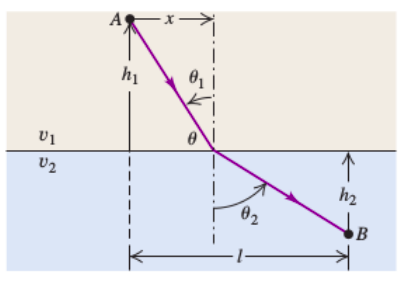
\includegraphics[width=.5\linewidth]{Imágenes/aux5/aux5pt2.png}
  \caption{Refracción}
  \label{fig:sub2}
\end{subfigure}
\caption{Donde el índice de refracción esta dada por $n=\frac{c}{v}$}
\label{fig:test}
\end{figure}

\begin{itemize}
    \item Mida cuando se demora la luz en llegar del punto inicial al final en función de la distancia y la velocidad de la onda.
    \item Derive con respecto a la posición en imponga que debe minimizarse como dice el principio de Fermat. ¿Qué condiciones se obtienen?.
\end{itemize}



\end{enumerate}
\end{document}